\documentclass[11pt]{article}

\usepackage{geometry, amsmath, amsthm, latexsym, amssymb, graphicx}
\usepackage{algorithm}  
\usepackage{algorithmicx}
\usepackage{algpseudocode} 
\usepackage{pgf}
\usepackage{tikz}
\usepackage{listings}
\usepackage{pythonhighlight}
\usepackage{subcaption}
\usepackage{float}
\usetikzlibrary{arrows,automata}
\geometry{margin=1in, headsep=0.25in}

\parindent 0in
\parskip 12pt

\begin{document}

\title{Correlation between score and gestures}

\thispagestyle{empty}

\begin{center}
    {\LARGE \bf Correlation between score and gesture}\\
\end{center}

\section{Score by gesture}
\begin{figure}[H]
    \centering
    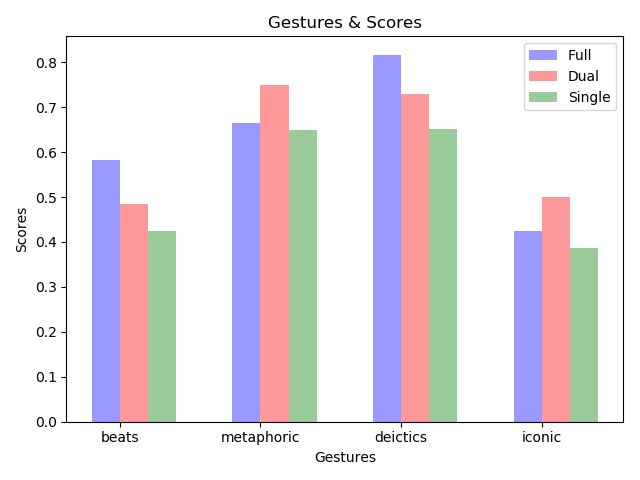
\includegraphics[scale=1]{correlation}
    \caption{Score by gesture}
    \label{}
\end{figure}

\section{split by type (infer/recall)}
\begin{figure}[H]
    \centering
    \begin{subfigure}[t]{0.5\textwidth}
        \centering
        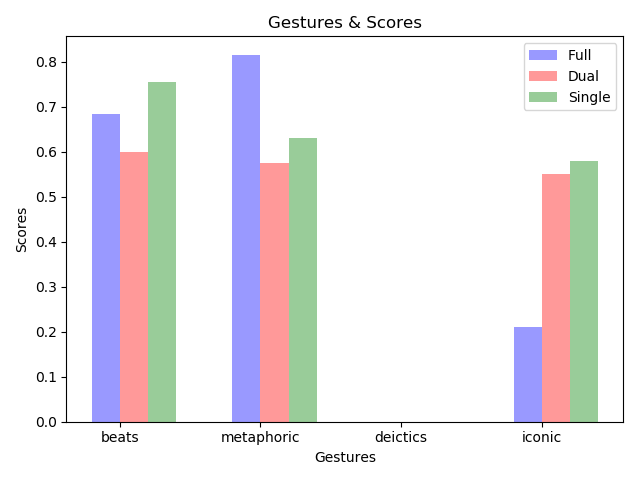
\includegraphics[scale=0.5]{infer}
        \caption{infer}
    \end{subfigure}%
    ~ 
    \begin{subfigure}[t]{0.5\textwidth}
        \centering
        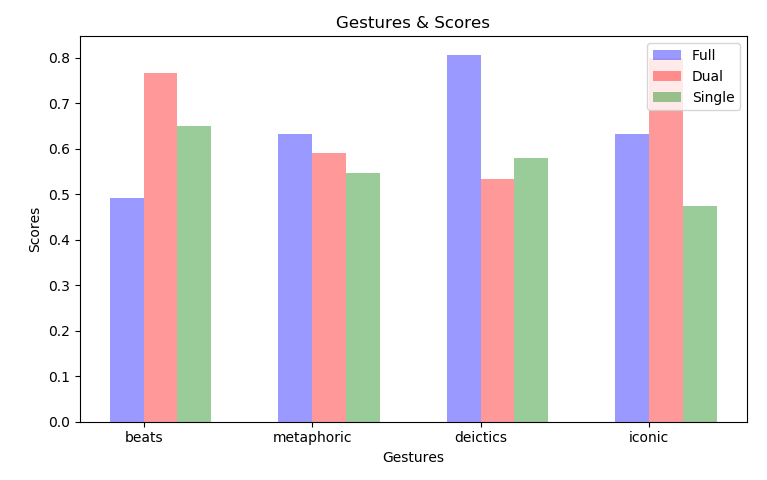
\includegraphics[scale=0.5]{recall}
        \caption{recall}
    \end{subfigure}
    \caption{Score by gesture}
\end{figure}

\section{split by difficulty (easy/hard)}
We can split the questions by the score under single condition. 
If the average score of one question below 0.5, we treat it as hard, otherwise, easy.

\begin{figure}[H]
    \centering
    \begin{subfigure}[t]{0.5\textwidth}
        \centering
        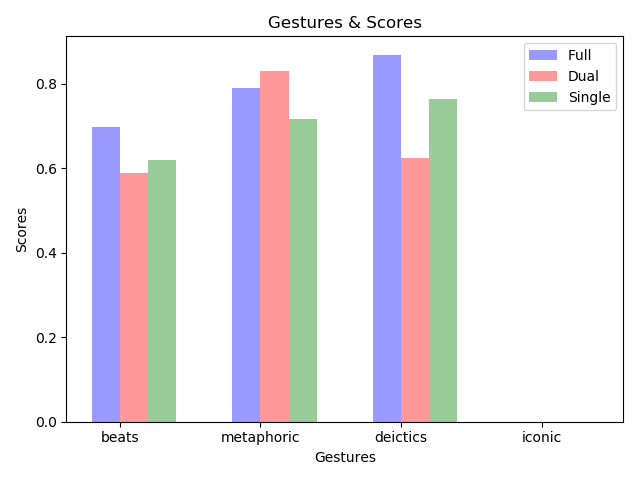
\includegraphics[scale=0.5]{easy}
        \caption{easy}
    \end{subfigure}%
    \begin{subfigure}[t]{0.5\textwidth}
        \centering
        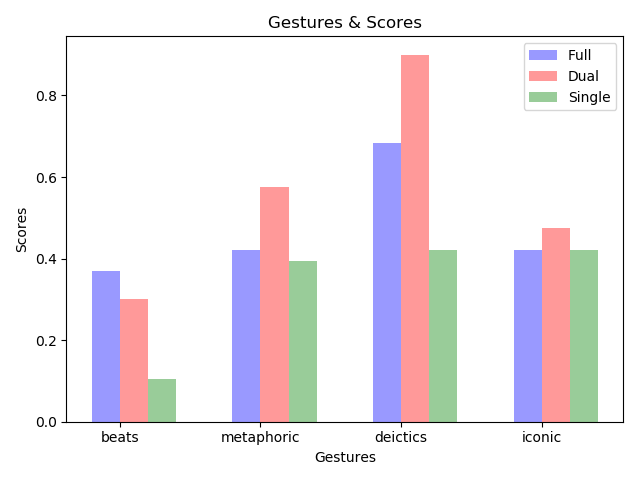
\includegraphics[scale=0.5]{hard}
        \caption{hard}
    \end{subfigure}
    \caption{Score by gesture}
\end{figure}

\section{18 Questions grouped by gestures:}

\begin{figure}[H]
    \centering
    \begin{subfigure}[t]{0.5\textwidth}
        \centering
        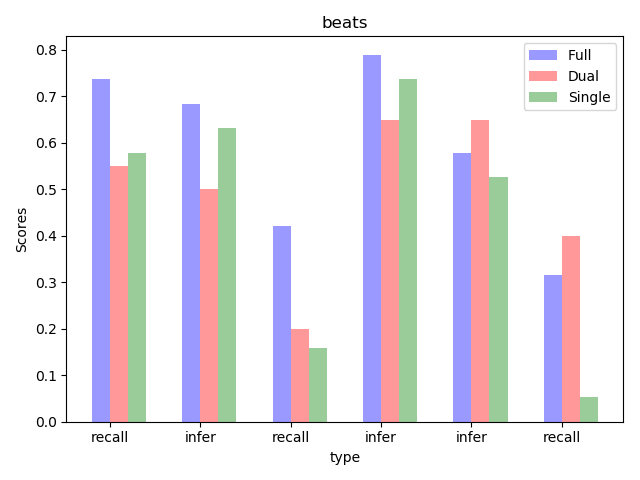
\includegraphics[scale=0.5]{beats}
        \caption{beat}
    \end{subfigure}%
    \begin{subfigure}[t]{0.5\textwidth}
        \centering
        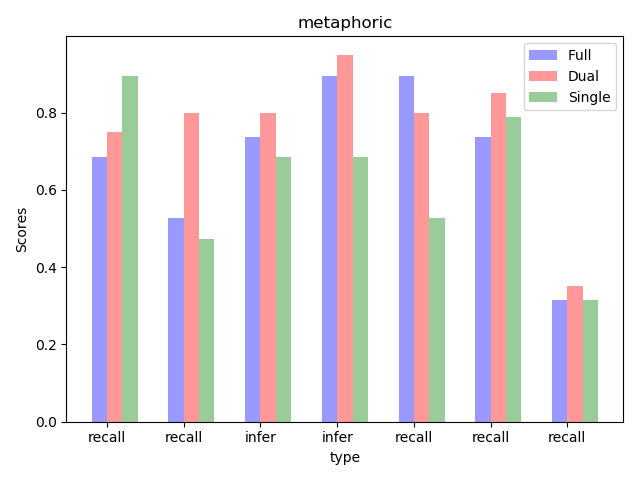
\includegraphics[scale=0.5]{meta}
        \caption{metaphoric}
    \end{subfigure}
    \begin{subfigure}[t]{0.5\textwidth}
        \centering
        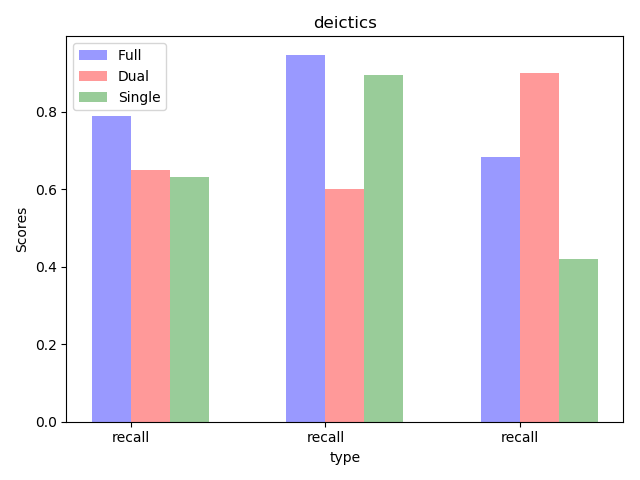
\includegraphics[scale=0.5]{deictics}
        \caption{deictic}
    \end{subfigure}%
    \begin{subfigure}[t]{0.5\textwidth}
        \centering
        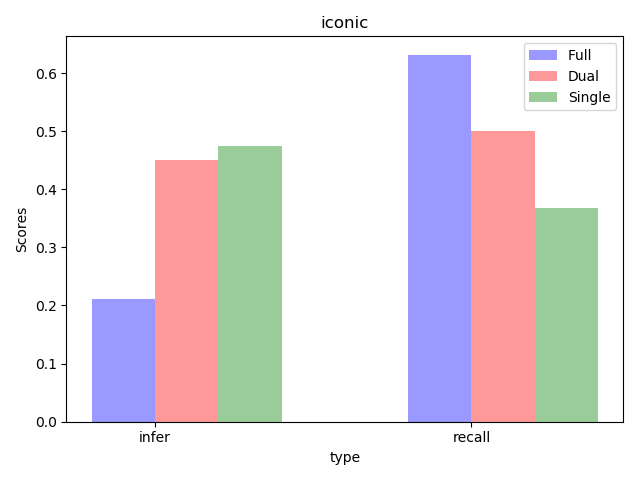
\includegraphics[scale=0.5]{iconic}
        \caption{iconic}
    \end{subfigure}
    \caption{Score}
\end{figure}

\end{document}